\section{Design}\label{design}


Developers using \sys{} write function handlers and define triggers just like
they would for any existing serverless offering. Additionally, developers
express jobs' priorities to \sys{}, and \sys{} enforces these priorities.



\subsection{Interface}

Developers express priorities to \sys{} via assigning functions to fixed
priorities that map directly to dollar amounts per unit compute. For instance in
the example of the web server, the home page view might be assigned a high
priority and cost 2c per cpu second, a the user profile view might be a assigned
a middle-high priority and cost 1.5c per cpu second, and finally the map reduce
job can be set to a low priority which costs only 0.5c per cpu second. This
enables the priorities to be globally comparable, while disincentivizing
developers to always choose the highest possible priority for their most
important job.
 
To avoid unexpected costs in the case of for example a DOS attack or a bug,
developers also express a monthly budget that they are willing to pay.\ \sys{}
uses this budget as a guideline and throttles invocations or decreases quality
of service in the case that usage is not within reason given the expected
budget, though it does not guarantee that the budget will not be exceeded by
small amounts.

Finally, developers are required to express a maximum amount of memory per
function.\hmng{ Should I have a forward reference to the discussion section
here? }



\subsection{\sys{} Design}

\begin{figure}[t]
    \centering
      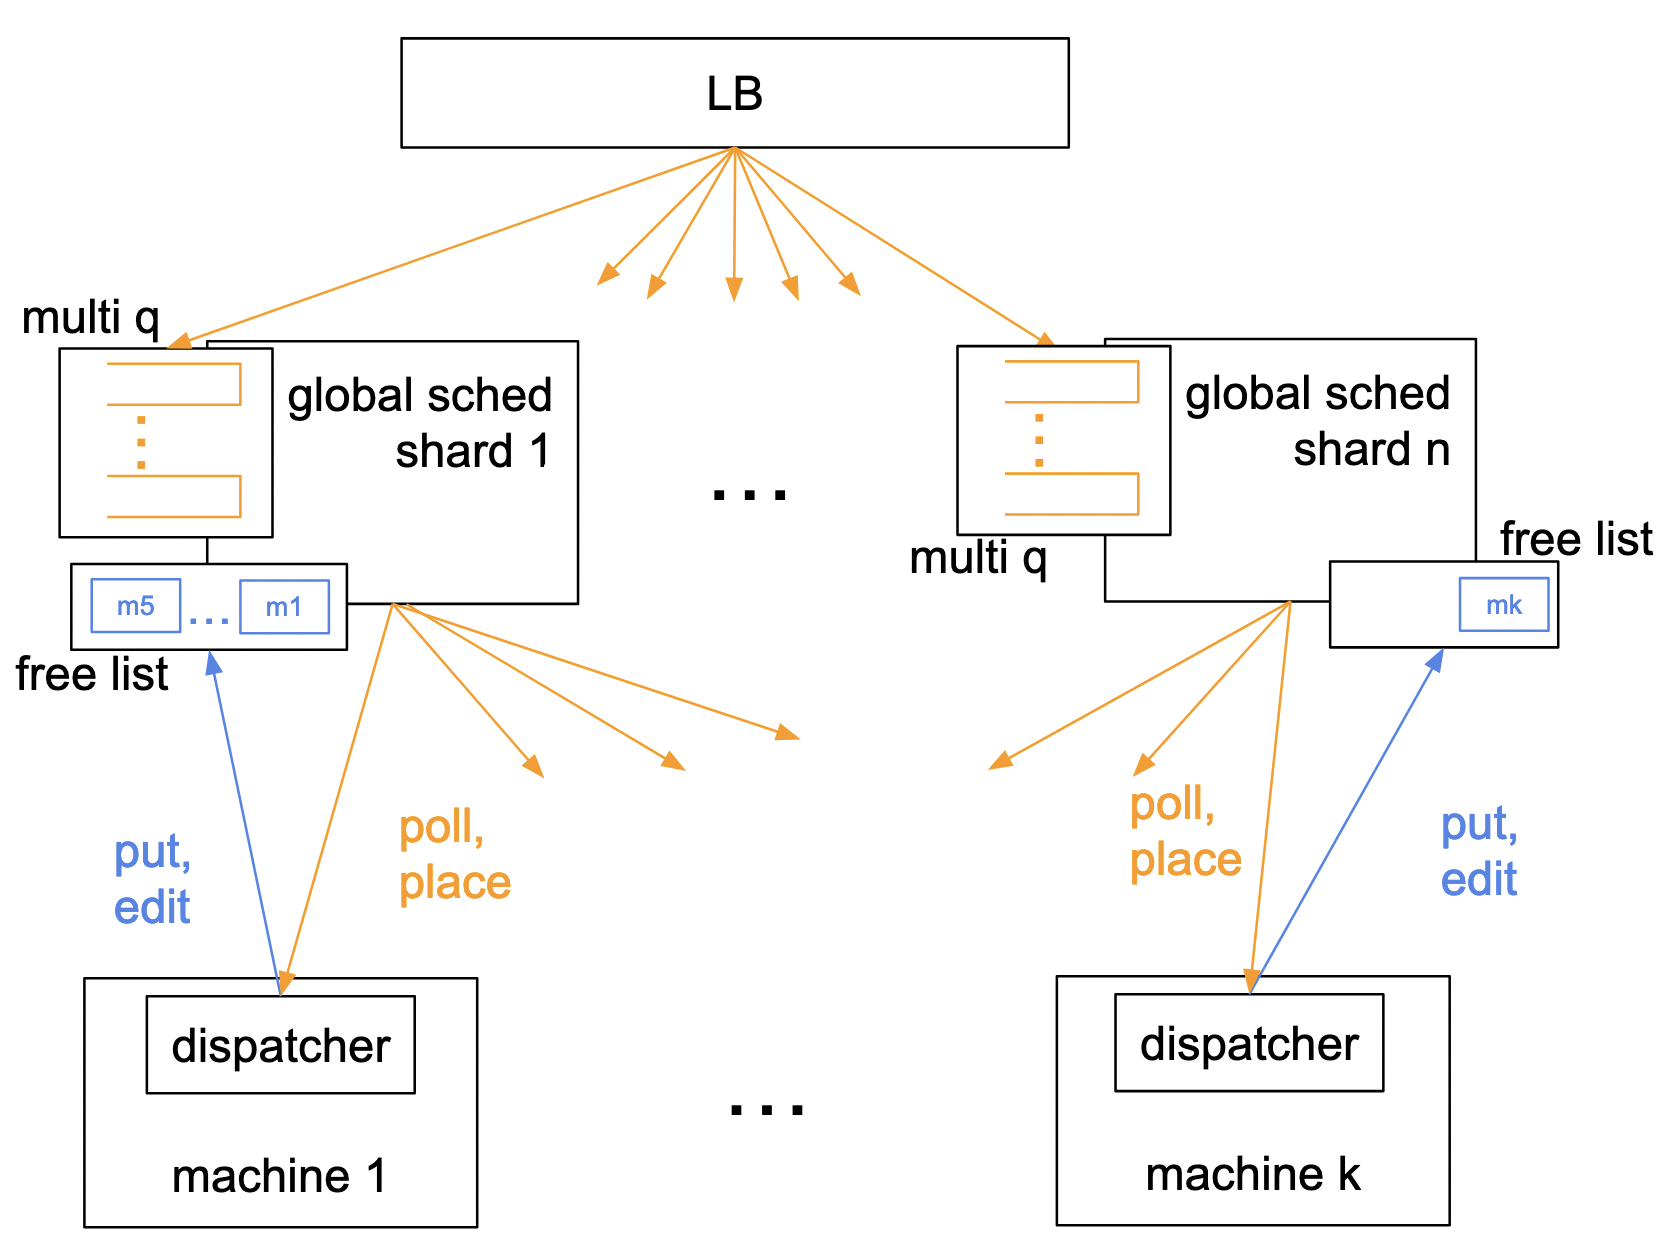
\includegraphics[width=9cm]{img/overview.png}
      \caption{ global scheduler shards queue and place jobs (in orange), 
      on each machine a dispatcher thread keeps track of memory utilization 
      and if it's low writes itself to a free list (in blue) }
    \label{fig:overview}
\end{figure}
  

\sys{}'s main structure can be seen in Figure\ref{fig:overview}: \sys{} consists
of a distributed global scheduler, which places new function invocations, a
dispatcher, which runs on each machine and communicates with the global
scheduler shards, and a machine scheduler, which enforces priorities on the
machines.

Attached to each global scheduler shard is an \textit{idle list}, which holds
machines that have a significant amount of memory available. In the shards idle
list each machine's entry is associated with the amount of free memory as well
as some information about compute pressure. This allows the global scheduler to
place high priority processes without incurring the latency overheads of finding
available resources.

The global scheduler stores the jobs waiting to be placed in a multi queue, with
one queue per priority.


\textbf{Machine Scheduler.}
The machine scheduler is simple: jobs have fixed priorities, and higher
priorities preempt lower priorities. Being unfair and starving low priority
jobs is desirable, since map reduce jobs should not interrupt a page view
request processing, but vice versa is expected.


\textbf{Dispatcher.}
The dispatcher is in charge of adding itself to a shard's idle list when memory
utilization is low. The dispatcher chooses which list to add itself to using
power-of-k-choices: it looks at k shards' idle lists and chooses the one with
the least other machines in it. If the machine is already on an idle list on
shard $i$, but the amount of available memory has changed significantly (either
by jobs finishing and memory being freed or by memory utilization increasing
because of new jobs or memory antagonists), the dispatcher will update shard
$i$'s idle list. These interactions from the dispatcher to free lists are
represented by the blue arrows in Figure\ref{fig:overview}.

The dispatcher also responds to probes by shards: given a potential job that a
shard might want to run on the machine, the dispatcher computes the \textit{time
to profit}, which is the time it would take for the machine to start making a
profit off of the decision of placing the job there. If there is enough memory
free to fit the new job's max memory, that number is 0. If the dispatcher might
have to kill a process due to memory pressure, it computes which job it would
kill, which is the job with minimal price where $j.memUsg > newJ.maxMem$. The
time to profit then is $(jToKill.timeRun \cdot jToKill.price) / (newJ.price
- jToKill.price)$.

The dispatcher is also in charge of killing jobs under memory pressure, should
it occur. It chooses the job to kill by looking at both memory used and money
wasted if killed (lower priority jobs should be the ones to be killed if
possible, but won't help much if they weren't using any memory to begin with).
The dispatcher requeues killed jobs at a randomly chosen shard.


\begin{algorithm}[t]
\caption{Choosing a machine for a job j}\label{alg:place}
\begin{algorithmic}
    \State$N = \{ $ machines in freeList with memAvail > j.maxMem $\}$
    \If{$|N| > 0$} \\
        \Return$ $min(N.maxPriorityRunning, N.qSize)
    \EndIf
    \State$M = $ timeToProfit of k polled machines
    \If{min(M.timeToProfit$) < THRESH$} \\
        \Return$ $min($M$)
    \Else
        \State$ $reQ j, with priority -= 1
    \EndIf
\end{algorithmic}
\end{algorithm}


\textbf{Global Scheduler.}

Shards choose what job to place next by the ratio of priority to amount of time
spent in the queue, so high priority jobs don't have to wait as long as lower
priority jobs to be chosen next.

When placing a job, the shard finds a machine to run the it, as also shown in
the pseudocode in Algorithm \ref{alg:place}. 

The shard will first look in its free list for a machine that has the job's
maximum memory available. If there are multiple such machines, the shard looks
at each machines compute pressure metrics; the goal being to minimize cpu
idleness and job latency in low load settings.\hmng{playing with deatils of this
in the scheduler right now} If a machine from the free list is chosen, the
response from the dispatcher on placing the job will include updated info,
which the shard will use to update the free list entry.

If there are no machines in the free list with the memory available, the shard
switches over to power-of-k-choices: it polls k machines, sending the price and
the maximum memory of the job currently being placed, and getting back the time
to profit. The shard then can choose to place the new job on the machine with
the minimum value, or if all of them are too high the shard re-queues the job,
this time with a lower priority.

Checking in with clients' budgets to ensure that usage is not significantly
outpacing a rate compatible with the budget is done asynchronously: each time a
job for a client is triggered a global counter is asynchronously updated. If the
counter's rate of change increases absurdly with regards to previous behavior as
well as the budget as a whole, this triggers a throttling for that job.
